\pdfoutput=1
\pdfminorversion=7
\documentclass{ecai}
\usepackage[T1]{fontenc}
\usepackage{graphicx}
\usepackage{amsmath,amssymb}
\usepackage{booktabs,tabularx}
\usepackage{microtype}
\usepackage[hidelinks,bookmarks=false]{hyperref}
\ecaisubmission
\hypersetup{pdftitle={GNOSIS: Continual Agent Repair with Activation Boundaries},pdfauthor={Zonghe Wu}}
\newcommand{\Gnosis}{GNOSIS}
\newcommand{\Global}{\texttt{GLOBAL}}
\newcommand{\E}{\mathbb{E}}
\newcommand{\Prob}{\mathbb{P}}
\newcommand{\ind}{\mathbf{1}}
\newtheorem{proposition}{Proposition}

\begin{document}
\begin{frontmatter}
\title{GNOSIS: Continual Agent Repair with Activation Boundaries}
\author[A,B]{\fnms{Zonghe}~\snm{Wu}\thanks{Corresponding author. Phone: 13646028118. Email: \nolinkurl{zonghe.wu@ucdconnect.ie}.}}
\address[A]{School of Architecture, Planning and Environmental Policy, University College Dublin, Belfield, Dublin 4, Ireland}
\address[B]{Chang'an-Dublin International College of Transportation, Chang'an University, Xi'an 710018, China}
\begin{abstract}
Persistent agent repair changes both future task behavior and the evidence needed to validate later updates. We introduce GNOSIS, a system that separates working and released versions and defines execution dependencies through activation boundaries: the first runtime event at which an edited component can influence an agent. Under pre-activation invisibility, coupled executions coincide until that event, making untouched historical trajectories reusable. The affected set of a release is the union of its component dependencies. On AutomationBench, four frozen agents are evaluated on 30 held-out tasks with five independent executions per task. GNOSIS achieves 67.33\% strict success, exceeding the fixed agent by 3.33 percentage points, and reduces frozen execution cost by 49.81\%. The task-paired comparison has a Holm-adjusted $p$-value of 0.656250. All delivered units have global scope, and all 48 validation plans require fresh executions; evidence reuse therefore saves zero executions. GNOSIS accepts two updates before selection scores saturate, while its development-inclusive cost remains above sequential revision across the observed 30 tasks. These results identify release locality and selection-feedback capacity as the structural conditions that govern the value of continual repair.
\end{abstract}
\end{frontmatter}

\section{Introduction}
\label{sec:intro}

An agent that improves through experience acquires obligations along with capabilities. A lesson learned while repairing a spreadsheet workflow can change how the agent interprets a later customer record. A new procedure for verifying a write can add calls to every future task. Each persistent update consequently changes the relationship between the deployed agent and the executions previously used to evaluate it. Continued improvement requires a way to determine which historical results remain applicable after an update.

This problem becomes concrete in enterprise automation. Tasks combine application programming interfaces (APIs) with business requirements whose satisfaction depends on the final state of several applications. AutomationBench evaluates such workflows through assertions over environment state~\cite{automationbench}. Operational experience can improve the discovery and use of these interfaces without changing model weights. StarHarness studies this form of adaptation by evolving the surrounding execution system~\cite{starharness}. Once updates accumulate, however, repeatedly evaluating every task consumes resources that could otherwise support additional repairs. The missing operational quantity is the dependency between a particular change and a particular execution.

A component's first opportunity to affect the agent gives that dependency a precise location. Consider a procedure that intervenes immediately before a specific endpoint is called. If the procedure is absent from the prompt and tool catalog before a matching call, all earlier decisions can remain identical across the old and new versions. An execution that never reaches the intervention point is outside the change's influence. This observation motivates the \emph{activation boundary}: the first registered runtime event matching any component in the change set. The boundary includes opportunities to alter tool arguments or observations, as well as context and workflow control.

\Gnosis{} uses this dependency in a continual repair workspace. A working version retains edits and receives feedback from development tasks. A released version advances only after the working version completes a source task and passes an independent selection comparison. Historical executions are then checked against the complete change set. Executions that encounter a changed activation condition are evaluated again; untouched evidence retains its original execution identity. The current AutomationBench adapter restarts affected tasks from their initial state. This gives an implementable form of selective validation without requiring restoration of intermediate model and environment states.

The central design tension lies in the unit of release. Components may be individually local, but a release combines their effects. Its validation set is the union of all affected executions. One global prompt edit therefore makes every historical execution relevant to the new release, even when the same release contains a narrowly applicable executable component. Figure~\ref{fig:architecture} connects the repair process to these local and global cases. The union rule makes locality a property of the entire change being accepted.

\begin{figure*}[t]
\centering
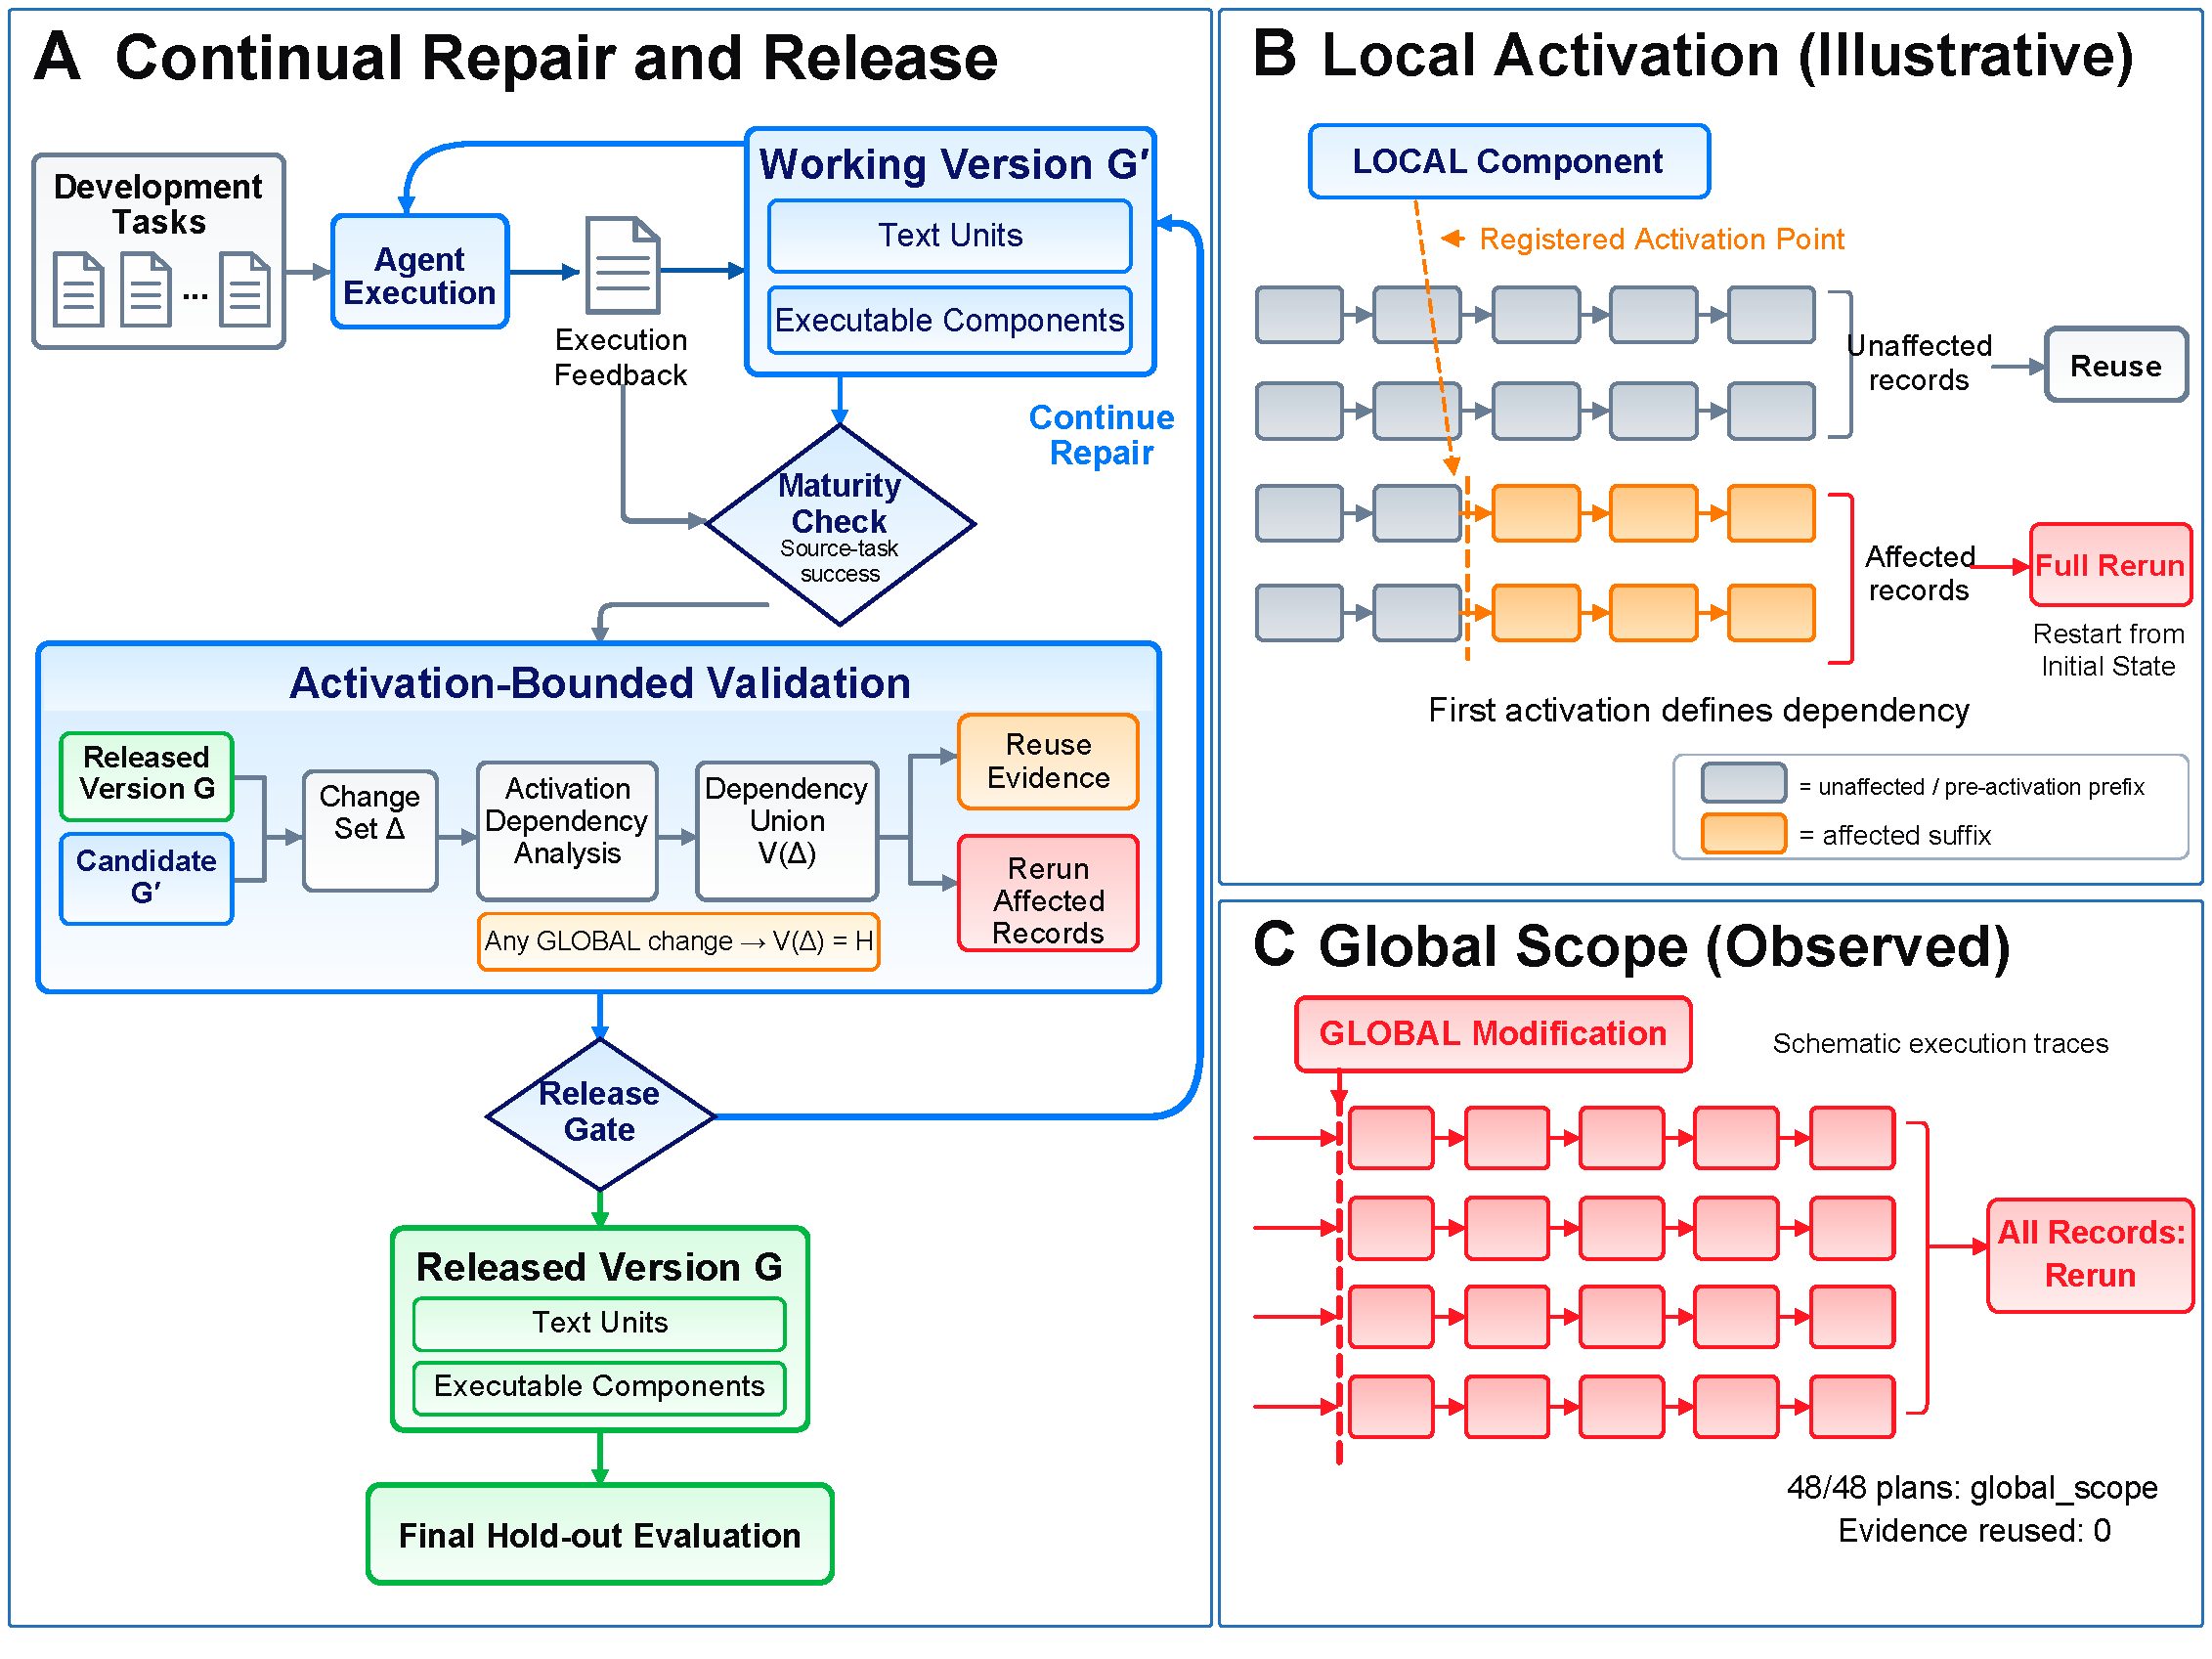
\includegraphics[width=0.96\textwidth]{figure1.pdf}
\caption{Continual repair and activation boundaries. A working version accumulates repairs, and a source-task success enables comparison with the released version. A local component remains invisible until a matching runtime event. Historical executions outside its influence can retain their evidence. A global change expands the affected set to all executions. The local path illustrates the mechanism; the evaluated releases followed the global path, with 48 of 48 GNOSIS validation plans requiring execution.}
\label{fig:architecture}
\end{figure*}

We examine three connected questions. RQ1 asks how persistent repairs change performance and execution expense on held-out workflows. RQ2 asks whether activation boundaries preserve usable evidence and reduce validation work. RQ3 asks how learning expenditure translates into accepted releases and task delivery under a comparable resource allocation. Four frozen agents are evaluated on the same 30 tasks, with five independent executions per task. A further comparison allocates GNOSIS's development and evaluation expenditure to sequential attempts on those tasks.

The resulting system achieves the highest observed strict success rate among the four frozen agents, 67.33\%, with 17 tasks succeeding in all five executions. Its frozen execution expense is 49.81\% below the fixed agent. At the same time, the evaluated updates expose the structural obstacle predicted by the union rule: every delivered unit has global scope, every mature comparison requires full candidate execution, and historical evidence reuse is zero. The strict-success difference against the fixed agent is 3.33 percentage points, with a task-paired 95\% interval of $[-4.00,10.00]$ and Holm-adjusted $p=0.656250$. These estimates define the observed performance result alongside the exact validation behavior.

The paper contributes an execution dependency definition with a coupling argument, a repair architecture that applies this definition to versioned evidence, and an empirical analysis connecting release scope to resource use. The analysis identifies two concrete constraints on further improvement. Global edits consume the entire validation set, and a selection set at its maximum score offers no further strict improvement signal. Both constraints arise within the repair process and directly determine how additional learning resources can be used.

\section{Related work}
\label{sec:related}

\subsection{Persistent experience with fixed model weights}

External experience changes agent behavior through several representations. Reflexion stores verbal feedback in episodic memory to improve later attempts~\cite{reflexion}. ExpeL extracts cross-task insights from successful and failed demonstration rollouts~\cite{expel}. Voyager accumulates executable skills that can be retrieved and composed in subsequent tasks~\cite{voyager}. Evo-Harness formalizes skill compilation by separating reflective lesson generation from structured executable constraints~\cite{evoharness}. These approaches establish text and code as persistent carriers of experience. The representation also determines where the experience enters execution: an instruction affects the decisions made with that instruction in context, while an executable skill introduces a particular callable behavior.

Agentic Context Engineering (ACE) maintains a structured playbook through generation, reflection, and incremental curation~\cite{ace}. SkillOpt optimizes skill documents through bounded edits informed by execution feedback~\cite{skillopt}. GEPA uses reflections over execution traces to guide prompt evolution~\cite{gepa}. GNOSIS permits both textual units and executable components within a versioned workspace. Its validation rule depends on when the changed unit becomes visible, so the same dependency definition applies to a retrieved instruction and to an operation that changes a tool call. Our ACE comparison uses its official reflection and curation implementation with the common execution model.

StarHarness evolves environment-specific execution systems and separates search from hidden selection and held-out evaluation~\cite{starharness}. GNOSIS adopts its benchmark adapter and deterministic improvement machinery. The continuous repair loop adds a persistent working version and requires complete source-task success before mature comparison. This arrangement keeps partial repairs available for further development while independently controlling advancement of the released version.

\subsection{Local control, composition, and execution dependencies}

EvoCUE installs experience as edits to an explicit state-machine controller and evaluates parent and edited continuations from the same checkpoint~\cite{evocue}. AutoHarness automatically synthesizes action verifiers that reject illegal actions before environment execution~\cite{autoharness}. In failure analysis across multi-step executions, Model or Harness? localizes the earliest unrecovered divergence along a trajectory to isolate model deficiency from tool and harness constraints~\cite{modelorharness}. GNOSIS studies a complementary dependency question: given a complete version change, which historical trajectories remain unchanged under a coupling of the executions? Pre-activation invisibility yields this criterion, and taking the union across edits extends it to an entire release. Our adapter evaluates affected tasks from the beginning; checkpoint continuation is outside the evaluated implementation.

CORDIS formalizes spatiotemporal composability using revertible effects and reactive coeffects~\cite{cordis}. It supplies a programming model for coordinating dynamic components and their dependencies. GNOSIS uses Cordis to register and manage executable plugins, with component code evaluated inside QuickJS. The historical evidence relation is defined by the agent runtime's activation events. Plugin composition provides the execution substrate on which that relation is enforced.

Regression test selection offers the closest software-engineering abstraction. Ekstazi tracks dynamic file dependencies to select tests after changes~\cite{ekstazi}. GNOSIS associates a historical execution with the runtime events it reaches. A change affects the execution when an old or new component can activate at one of those events. This handles newly introduced components by testing their activation conditions against existing traces. The dependency includes information exposed to the model, which makes prompt visibility and tool discovery part of the execution contract.

\subsection{Acceptance and resource allocation}

SAGE evaluates candidate updates through paired outcomes and a statistical acceptance rule~\cite{sage}. GNOSIS records SAGE statistics on mature comparisons while using the StarHarness improvement decision with a zero-regression condition for publication. Acceptance and evidence selection thus have distinct roles: the first determines whether an update advances the released version; the second determines which executions must be performed to supply that comparison.

Evaluation of persistent adaptation also requires the cost of obtaining experience. \emph{Rethinking the Evaluation of Harness Evolution for Agents} argues for matched feedback and inference budgets together with held-out tasks~\cite{rethinking}. We separate frozen execution expense from development expenditure and include sequential revision as an alternative allocation of the latter. This accounting connects the benefit of a persistent version to the number of tasks over which its acquisition cost is shared. It also exposes whether an apparent resource advantage occurs during deployment, validation, or the complete evaluated process.

\section{GNOSIS: repair and validation through activation boundaries}
\label{sec:method}

\subsection{Versioned continual repair}

Let $G$ denote an ordered collection of persistent experience units used by an agent with fixed model parameters. GNOSIS maintains three version references: a working version $W$, a released version $R$, and a frozen version $F$ used for final evaluation. An edit creates an immutable collection and moves $W$ to it. Development execution produces task outcomes and traces associated with that exact version. Acceptance moves $R$ to $W$; freezing sets $F=R$ and closes learning. The separation prevents an unsuccessful intermediate repair from replacing the released behavior.

The repair model operates on actual development evidence. It can inspect an authorized task's trajectory, edit the collection, and execute another development task. The resulting failure or success returns to the same repair process. For example, correcting pagination may reveal that a required notification remains unsent. Keeping both edits in the working version allows the process to complete the workflow without discarding the earlier correction. The source task must satisfy every strict assertion before the current working version can enter mature comparison. Any subsequent edit invalidates that maturity record because it creates a different candidate.

A mature candidate is compared with the released version on a separate selection set. A rejected comparison leaves the released version in place and returns selection feedback to the repair model. The working version remains available for further edits. This makes the selection set an adaptive development resource with a distinct role from the final held-out tasks. Those final tasks are evaluated only after versions have been frozen, and their outcomes never enter repair messages.

\begin{figure}[t]
\hrule\smallskip
\small
\noindent\textbf{Algorithm 1: Continual repair with activation boundaries}
\begin{enumerate}
\setlength{\itemsep}{2pt}
\item Initialize working and released collections $W=R$ and an evidence store $\mathcal H$.
\item Inspect authorized development evidence and edit $W$; clear the source-success marker after each edit.
\item Execute a development task using $W$. Retain its result and return feedback to the repair process.
\item If the current $W$ has completed a source task, permit a mature comparison. Obtain selection evidence for $R$ and compute $\Delta=\operatorname{diff}(R,W)$.
\item For each reference execution $h$, evaluate $W$ from task start if $h\in\mathcal V(\Delta)$; otherwise carry its evidence forward with the source execution identity.
\item Apply deterministic improvement and zero-regression conditions to the paired results. Advance $R\leftarrow W$ on acceptance.
\item Continue repair until the learning process stops or its group allowance is exhausted. Freeze $F\leftarrow R$.
\end{enumerate}
\smallskip\hrule
\end{figure}

\subsection{Experience units and the runtime contract}

Each unit contains an identifier, an activation scope, a set of runtime hooks, and textual experience. An optional component type and TypeScript source add executable behavior. A local scope names services, endpoints, or tools. The special scope \Global{} is exclusive: it cannot be combined with local scope entries in the same unit. Version identity covers the collection and its order, so changing the order of retained units participates in dependency analysis.

The runtime registers events at task start and at tool discovery, before and after tool calls, and at context, workflow, and operation hooks. Each event identifies its hook and the applicable service, endpoint, or tool. A unit is eligible when its hook is registered for that event and its scope matches the event identity. These matches concern API identities and runtime structure. The model supplies the experience and chooses its intended scope during repair.

Local units remain invisible until a matching event. Before activation, their contents do not enter model prompts or alter the tool catalog, and the host does not load their plugin. After activation, the hook constrains their available interventions. Arguments can change before a call; returned observations can change after it; context and workflow hooks can supply messages. Executable operations become callable only after activation. Successful responses and error observations pass through the same registered observation path, and discovered endpoints generate discovery events. This coverage makes failed interaction attempts part of the dependency trace.

The host compiles component source and registers it as a Cordis plugin~\cite{cordis}. QuickJS execution and operating-system isolation constrain the component to the capabilities of the current task. A component can request the task's existing API operations and consume their results; permissions and the benchmark evaluator remain outside its control. Runtime records distinguish loading a plugin from an intervention that changes execution. An invocation with no effect is still a component invocation, but it contributes no observed argument, context, or capability change.

The final GNOSIS collection contains 13 textual units and one executable component, \texttt{ace\_op\_vp\_guard}. The latter handles position information at the API argument interface. This component demonstrates where a repair can be installed within the runtime. Its invocation and intervention counts are examined separately in Section~\ref{sec:scope-results}, so the empirical explanation follows the behavior that actually occurred.

\subsection{Activation boundaries and reusable evidence}
\label{sec:boundary}

Let $G$ be a released version and $G'$ a candidate. The change set $\Delta$ includes additions and deletions, together with both old and new forms of modified units. Changes to scope or relative order are included. Write a trajectory's registered events as $e_0,e_1,\ldots$, and let $a_u(e)$ indicate whether unit $u$ can activate at event $e$. The first activation boundary is
\begin{equation}
b^*(\tau,\Delta)=\inf\{k:\exists u\in\Delta,\ a_u(e_k)=1\},
\label{eq:boundary}
\end{equation}
with $b^*=\infty$ if the set is empty. Considering both old and new activation conditions detects effects removed by a deletion as well as effects introduced by an addition.

The boundary property rests on three assumptions. First, the task's initial state and the model and environment transition laws are fixed across versions. Second, changed units have no influence before their first eligible event, and all influence paths pass through the registered runtime. Third, the mathematical comparison couples model and environment randomness across executions. Removing the first assumption changes the underlying process. Removing the second permits divergence before the recorded boundary. Removing the coupling removes sample-path equality. Independent API executions in the experiment use task pairing for statistical analysis; the common-randomness construction is used for the property below.

\begin{proposition}[Pre-activation invariance]
Under these assumptions, executions of $G$ and $G'$ with the same random source have identical states and observations before $b^*$. If $b^*=\infty$ on the execution of $G$, the complete coupled trajectories and their scores are identical.
\label{prop:invariance}
\end{proposition}

Before the first eligible event, neither version exposes the changed units. Identical inputs and coupled randomness produce identical model actions, while equal environment transitions produce the same observations and next events. Induction extends this equality until activation or termination. In particular, a new unit cannot generate its own earlier trigger without first influencing an execution, which the invisibility condition excludes. Appendix~\ref{app:proof} provides the detailed argument.

Let $A_\Delta$ denote the event that an execution reaches a changed activation condition, and let the task score $Y$ lie in $[0,1]$. The same coupling yields
\begin{equation}
\left|\E_{G'}[Y]-\E_G[Y]\right|
\leq \Prob_G(A_\Delta).
\label{eq:bound}
\end{equation}
Outside $A_\Delta$, Proposition~\ref{prop:invariance} makes the score difference zero. Inside it, the absolute difference is at most one. The probability of reaching the change therefore bounds the maximum change in expected score. This is a dependency bound for a fixed version pair; it does not require estimating that probability from a validation batch.

For a historical evidence collection $\mathcal H$, define the affected set of a unit and of the complete change as
\begin{align}
\mathcal I(u)&=\{h\in\mathcal H:\exists e\in h,\ a_u(e)=1\},\\
\mathcal V(\Delta)&=\bigcup_{u\in\Delta}\mathcal I(u).
\label{eq:union}
\end{align}
An untouched record describes the same execution under the candidate when coupled to its original random source. GNOSIS preserves that record with its originating execution identity. This transfer does not create another independent observation. The provenance is part of the candidate's evidence, and repeated use of the record retains that dependence.

Global edits are conservatively assigned $\mathcal I(u)=\mathcal H$ by the validation planner. Thus one changed global unit implies $\mathcal V(\Delta)=\mathcal H$. Missing boundary traces also require execution, while an incompatible program or source-version identity prevents a record from serving as reference evidence. These rules give every reusable record a specific version and a trace on which absence of influence was checked.

\subsection{Mature selection and validation expense}
\label{sec:selection}

The selection set contains six tasks, with two executions per task on each side of a comparison. Reference evidence is indexed by the released version and is retained for subsequent comparisons of that version. Candidate evidence is assembled by applying Equation~\eqref{eq:union}. Each affected record causes one fresh execution from task start. An unaffected record is carried forward without a new API execution. The global-validation control follows the same repair process and always executes the candidate side in full.

For candidate execution costs $c_h$, the direct candidate validation expense is
\begin{equation}
C_{\mathrm{candidate}}(\Delta)=\sum_{h\in\mathcal V(\Delta)}c_h.
\label{eq:cost}
\end{equation}
The complete comparison also includes any reference evidence that must be obtained and other actual calls. Equation~\eqref{eq:cost} prices whole executions because the adapter has no complete intermediate-state restoration interface. The first boundary determines whether execution is required and records the potential starting point for a future continuation mechanism.

Publication combines the StarHarness deterministic improvement and promotion decisions with zero regression on paired task outcomes. Mean strict success and per-task success rates enter the improvement check, with mean partial credit available to its verifier criterion. For regression, a task is solved only if both executions succeed; a previously solved task becoming unsolved counts as a loss. A candidate advances the released version only when the improvement checks pass and the loss count is zero.

The same evidence also produces SAGE paired statistics with penalty one and one-sided significance level 0.05~\cite{sage}. These statistics accompany the comparison. With six selection tasks, five wins and zero losses are required for the paired sign test to reach that level. Using deterministic improvement for publication allows smaller complete repairs to advance while retaining an explicit record of the statistical evidence. This choice also gives the selection process a finite ceiling: once both strict success and the verifier score are maximal, further candidates have no improvement margin on that set.

\section{Experimental design}
\label{sec:design}

\subsection{Tasks and shared execution conditions}

AutomationBench is fixed at commit \texttt{4a8e106}, using its original API tools and strict final-state assertions~\cite{automationbench}. The task split uses seed 100, with 30 development tasks, six independent selection tasks, and 30 held-out tasks. Each split covers six business domains. Six development tasks, one per domain, also serve as a retention checkpoint. The checkpoint outcomes are stored separately and excluded from repair feedback. Appendix~\ref{app:protocol} specifies the task identities and frozen versions.

The execution and repair model is the official DeepSeek API model \texttt{deepseek-flash}. Thinking is enabled, reasoning effort is high, temperature is one, and each execution has at most 50 agent steps. The configured maximum output is 393,216 tokens per model response; the model context capacity is 1M tokens. Reasoning content is retained across tool-call rounds. These settings are fixed for all groups. A development execution check completes all 30 tasks, succeeds on 21, and records no output truncation among the nine failures, satisfying the execution condition for learning to begin.

Each frozen group performs five independent executions per held-out task, for 150 executions per group and 600 in total. Every execution initializes the task environment and component state anew. The input does not contain a previous held-out answer or its feedback. Comparability therefore depends on common initial states and scoring contracts, while transfer depends on excluding held-out evidence from learning. Removing either condition changes the interpretation of the group comparison. All 600 frozen evaluations terminate normally under the execution protocol; strict failure still occurs when final-state assertions are unsatisfied.

\subsection{Comparison groups and resource allocation}

The \emph{Fixed} agent has no learned experience units. \emph{ACE} uses the official reflector and curator to maintain textual experience~\cite{ace}. \emph{Global} uses the GNOSIS repair workspace with full candidate validation. \emph{GNOSIS} applies activation-based evidence selection in that workspace. Global and GNOSIS share the same learning allowance, USD~8.5 at the experiment's reference prices. Fixed and ACE have allowances of USD~2 and USD~3, respectively. These are limits on settled learning and selection expenditure; unused allowance remains unused when a learning process stops.

The allowances define the comparison conditions, and actual settled expense determines resource use. Global spends USD~3.028831 on learning and selection, and GNOSIS spends USD~4.310552. The two groups follow their own candidate trajectories, with four mature comparisons each. ACE's final playbook is represented as one textual unit; Global freezes 17 textual units, and GNOSIS freezes 14 units in total. Final evaluation uses each group's released collection after freezing.

The \emph{Repeat} condition allocates GNOSIS's development-plus-held-out expense equally across the same 30 held-out tasks. Within a task, successive attempts receive the preceding process for revision, and the final attempt determines its score. The allocation includes GNOSIS's learning, selection, and checkpoint expense together with its five-execution held-out evaluation. Fixed-candidate retests are excluded from this allocation and reported separately. Repeat uses 354 attempts overall and produces 30 final outcomes.

\subsection{Outcomes and statistical analysis}

The primary endpoint is strict success. For task $i$ and group $g$, $\bar Y_{ig}$ is the fraction of its five independent executions satisfying all benchmark assertions. Group differences are means of the 30 paired task differences. A two-sided exact paired permutation test enumerates all sign assignments of nonzero differences. Confidence intervals use 200,000 paired bootstrap resamples of tasks with random seed 100. Holm correction applies to the three primary GNOSIS-versus-control comparisons.

Partial credit is averaged over the five executions within each task. A second task outcome records whether all five executions succeed, and paired differences in this binary outcome use the two-sided exact McNemar test. Each secondary endpoint has its own three-comparison Holm family. Retaining the task as the statistical unit preserves the shared task structure of repeated executions. Repeat's final-attempt endpoint is reported as the delivery outcome of its sequential allocation, alongside the independent-execution average of the frozen agents.

\subsection{Cost definitions}

Reference expense is computed from settled token usage at CNY~1 per million uncached input tokens, CNY~0.02 per million cached input tokens, and CNY~4 per million output tokens. USD allowances use CNY~7.1 per USD. Frozen execution cost covers only the 150 held-out executions of a group. Development cost includes learning and selection, plus the retention checkpoint where present. Total experimental cost additionally includes fixed-candidate retests. Unsettled reservations are excluded from these totals.

The provider export supplies aggregate cash expenditure, while the local call ledger supplies group and phase attribution. The export contains 18,467 requests totaling CNY~206.71348282. Local settled reference expense is CNY~203.837800, leaving CNY~2.875683 at aggregate level. The export has daily totals without a request-to-group mapping. Appendix~\ref{app:cost} provides the usage categories and daily amounts, keeping the provider total and the experimental group accounting explicit.

\section{Results}
\label{sec:results}

\subsection{RQ1: held-out performance and frozen execution cost}

GNOSIS achieves 101 strict successes in 150 held-out executions, or 67.33\%, the highest observed rate among the four frozen versions (Table~\ref{tab:main}). It exceeds Fixed by 3.33 percentage points, ACE by 8.00, and Global by 5.33. The corresponding task-paired 95\% intervals are $[-4.00,10.00]$, $[-2.67,19.33]$, and $[-2.00,12.67]$ percentage points. All three Holm-adjusted $p$-values are 0.656250. The observed ranking favors GNOSIS; the primary comparisons do not reach the 0.05 significance threshold.

\begin{table*}[t]
\centering
\caption{Held-out outcomes and settled reference expense. Each frozen agent has 150 executions on 30 tasks. Repeat has 30 final outcomes after 354 sequential attempts. All-five counts apply to the frozen groups. Costs are CNY, rounded here to three decimals; Appendix~\ref{app:cost} gives phase details. Total expense includes development and fixed-candidate retests where present.}
\label{tab:main}
\begin{tabular}{lrrrrr}
\toprule
Group & Strict success (\%) & Partial credit & All five / 30 & Held-out cost & Total cost\\
\midrule
Fixed & 64.00 & 0.857796 & 10 & 28.279 & 34.339\\
ACE & 59.33 & 0.849316 & 11 & 24.112 & 34.283\\
Global & 62.00 & \textbf{0.905716} & 12 & 17.351 & 41.256\\
GNOSIS & \textbf{67.33} & 0.905183 & \textbf{17} & \textbf{14.194} & 48.128\\
\midrule
Repeat & 53.33 & 0.733767 & --- & 45.832 & 45.832\\
\bottomrule
\end{tabular}
\end{table*}

The task matrix in Figure~\ref{fig:matrix} shows how repeated success is distributed. Seventeen GNOSIS tasks succeed in every execution, compared with ten for Fixed, eleven for ACE, and twelve for Global. Against Fixed, eight tasks move into the all-five category and one moves out. The exact McNemar $p$-value is 0.039063 before correction and 0.117188 after correction. Appendix~\ref{app:statistics} reports the complete paired results. The all-five outcome emphasizes consistent completion within a task and complements the mean success rate.

\begin{figure*}[t]
\centering
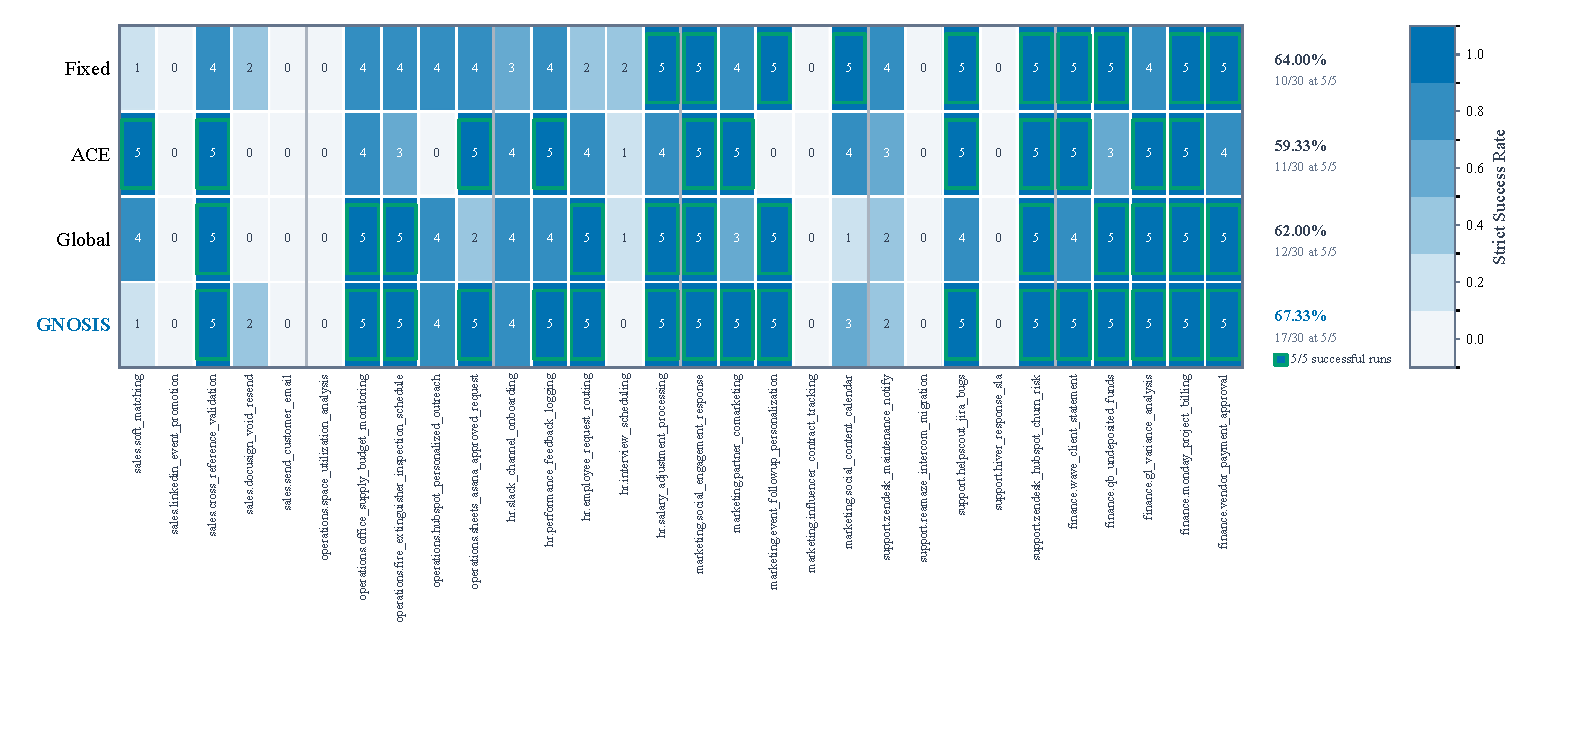
\includegraphics[width=\textwidth]{figure2.pdf}
\caption{Strict success by held-out task and frozen group. Each cell is the success fraction from five independent executions. The matrix retains the task structure used in paired statistical analysis and shows the distribution of tasks that succeed in all five executions.}
\label{fig:matrix}
\end{figure*}

Partial credit describes a different part of task completion. Global has the highest average, 0.905716, followed by GNOSIS at 0.905183. GNOSIS's difference from Fixed is 0.047386, with a task-paired 95\% interval of $[0.012508,0.085662]$ and adjusted $p=0.050743$. The gap between partial and strict success reflects the requirement that every assertion hold for a complete workflow. A system can satisfy most requirements on many tasks while missing the final condition needed for strict success.

GNOSIS also has the lowest frozen execution expense, CNY~14.194113. Relative to Fixed, ACE, and Global, the reductions are 49.81\%, 41.13\%, and 18.19\%, respectively. Its average held-out execution costs CNY~0.094627, compared with CNY~0.188528 for Fixed. These amounts price task execution after learning has ended. Adding development and retesting brings GNOSIS's total to CNY~48.128490, the highest of the four frozen groups. The expenditure split locates the observed economy in deployment execution.

\subsection{RQ2: global changes eliminate reusable evidence}
\label{sec:scope-results}

Every delivered experience unit has \Global{} scope. Across GNOSIS's four mature comparisons, all 48 candidate validation plans select the global-scope path, with first boundary zero and restart at task start. Each comparison therefore performs 12 candidate executions and reuses zero records. Equation~\eqref{eq:union} predicts this behavior directly: a global member of the change set includes every reference execution in the affected union.

Two fixed candidate pairs provide a further comparison of validation modes. One pair comes from Global and one from GNOSIS. Each pair is evaluated using both activation-based selection and full validation. Both modes abstain on both pairs, yielding decision agreement of two out of two. Each candidate side performs 12 executions and reuses none (Table~\ref{tab:retest}). Execution savings are exactly zero.

\begin{table}[t]
\centering
\caption{Fixed-candidate retests. Scoped and full validation both abstain for each pair. Counts are candidate executions / reused records; expense is candidate execution cost in CNY.}
\label{tab:retest}
\small
\begin{tabular}{lrr}
\toprule
Candidate source & Scoped & Full\\
\midrule
Global: execution / reuse & 12 / 0 & 12 / 0\\
Global: cost & 1.094279 & 1.306276\\
GNOSIS: execution / reuse & 12 / 0 & 12 / 0\\
GNOSIS: cost & 0.996941 & 0.859561\\
\bottomrule
\end{tabular}
\end{table}

The two modes still incur different token expenses because they perform separate complete executions. Scoped validation costs CNY~0.211997 less for the Global pair and CNY~0.137379 more for the GNOSIS pair. With identical execution counts and no reused record, these differences arise from the usage of the fresh executions. The reuse mechanism contributes zero to the measured savings.

Runtime behavior further distinguishes executable availability from executable influence. The final GNOSIS guard is invoked 6,276 times across the 150 held-out executions, including 150 task-start invocations and 6,126 before-call invocations. It produces zero recorded interventions and zero capability calls. The 13 textual units are injected 1,950 times in total. The evaluated version thus supplies persistent textual guidance throughout held-out execution while its executable guard remains behaviorally inactive. Local pre-activation behavior has an offline check on one synthetic component; the learned releases exercise the global validation case.

\subsection{RQ3: accepted releases and selection saturation}

GNOSIS accepts two updates, compared with one for Global. Dividing by settled learning and selection expense gives 0.463978 accepted releases per USD for GNOSIS and 0.330160 for Global, a 40.53\% increase. Both groups make four mature comparisons and execute 48 candidate records. The higher acceptance density occurs with equal validation execution counts and no evidence reuse. It reflects the accepted updates obtained along the two learning trajectories.

The selection outcomes expose the stopping condition. GNOSIS advances the released mean from $10/12$ to $11/12$ and then to $12/12$. Global advances from $10/12$ directly to $12/12$. Their last comparisons both have a candidate mean of one and a released mean of one, and both abstain. At that point the current selection scores provide no further strict improvement. Global retains USD~5.471169 of its allowance and GNOSIS retains USD~4.189448. Figure~\ref{fig:cost} places accepted releases against cumulative settled expenditure, locating the steps at their actual acceptance events.

\begin{figure*}[t]
\centering
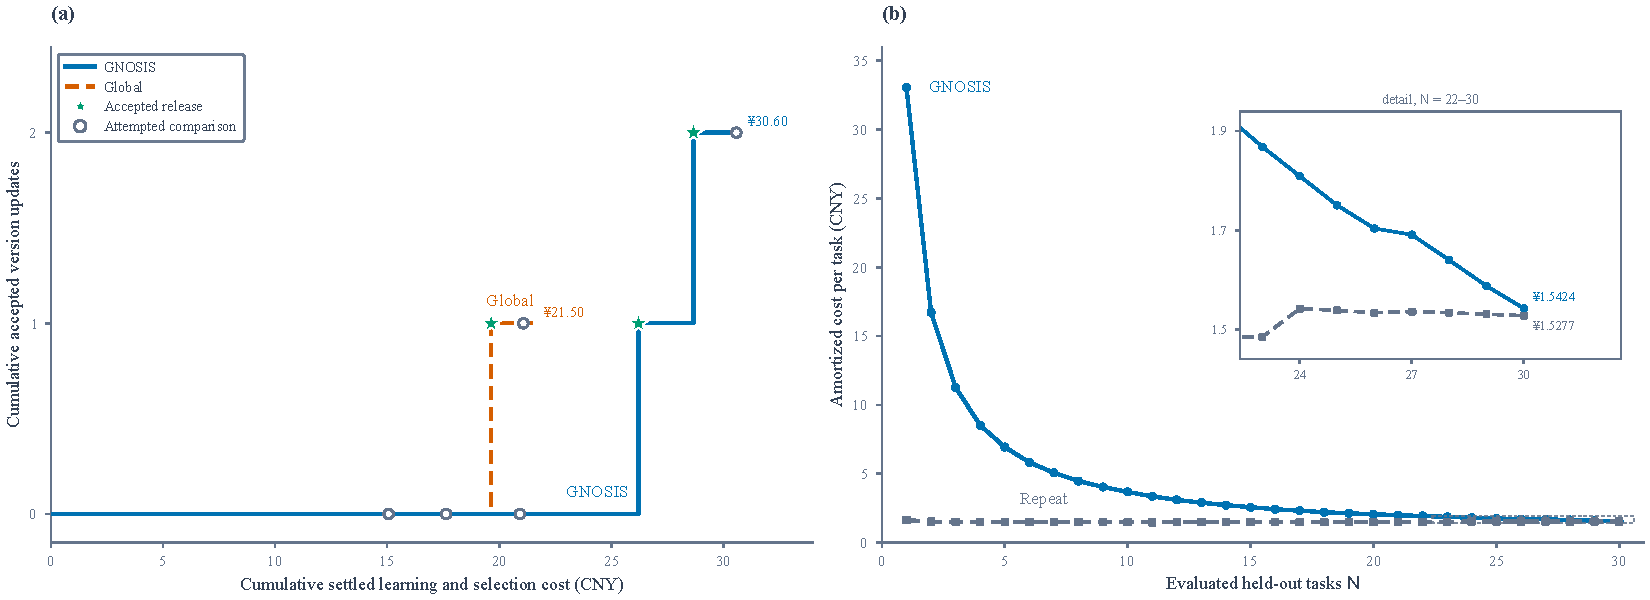
\includegraphics[width=\textwidth]{figure3.pdf}
\caption{Learning and amortized expense. Left: accepted releases against cumulative settled learning and selection expense, with steps at the recorded acceptance events. Right: development-inclusive expense per task for GNOSIS and sequential revision, accumulated in the fixed held-out task order. GNOSIS's evaluation term includes five independent executions per task. The observed curves do not intersect within 30 tasks.}
\label{fig:cost}
\end{figure*}

\subsection{Sequential revision and amortized expense}

GNOSIS spends CNY~46.271988 on development plus held-out evaluation. Repeat spends CNY~45.831735, 0.95\% below the allocated amount. Under this near-equal resource allocation, GNOSIS's strict success is 67.33\% and Repeat's final-result success is 53.33\%, a difference of 14.00 percentage points. Repeat's mean partial credit is 0.733767. The two endpoints follow the allocation policies: GNOSIS averages five independent deliveries per task, and Repeat scores the last delivery after sequential revision.

Let $D$ denote GNOSIS's development expenditure, $c_i$ the cost of all five independent evaluations of held-out task $i$, and $r_i$ the cost of its sequential attempts. In the fixed task order, the observed amortized costs are
\begin{equation}
A_G(n)=\frac{D+\sum_{i=1}^{n}c_i}{n},\qquad
A_R(n)=\frac{\sum_{i=1}^{n}r_i}{n}.
\label{eq:amortization}
\end{equation}
At $n=30$, these are CNY~1.542400 and CNY~1.527725 per task. The GNOSIS curve remains above the Repeat curve for every observed prefix from one to 30 tasks. The evaluated allocation achieves a higher final success rate with persistent experience and has no observed cost crossover. The five-execution cost term is retained explicitly, so this curve describes the evaluated resource allocation.

\subsection{Retention during repair}

The six-task development checkpoint improves from four strict successes to five. Two tasks change from failure to success, and one changes from success to failure. Partial credit rises from 0.934524 to 0.958333. This pattern shows that an improving aggregate can coexist with a loss on an individual earlier task. The checkpoint uses a working candidate distinct from the final frozen release; Appendix~\ref{app:components} identifies both versions. Maintaining separate working and released references assigns this intermediate behavior to the candidate that produced it.

\section{Discussion}
\label{sec:discussion}

\subsection{Release locality is the resource that selective validation uses}

The zero-reuse result follows from the granularity of accepted change. GNOSIS supports activation conditions tied to particular runtime events, yet the evaluated learning process delivers globally scoped units. The validation planner consequently includes every execution. This behavior reveals a design requirement for productive selective validation: a mature release must preserve locality across its entire change set. A local executable edit packaged with global textual revisions has global validation expense.

The union rule also explains why counting local components alone is an inadequate measure of available savings. Two narrow components may jointly reach nearly every task, while several changes confined to the same small workflow may share one affected set. The relevant quantity is the coverage of the union on reference executions. Exposing that coverage to the repair process would make the resource consequence of an edit explicit. Source-task success remains the maturity requirement, and the estimated validation workload becomes part of choosing how to assemble a complete repair.

This leads to a specific architectural direction: construct mature changes whose activation conditions capture the operational dependency actually repaired. A procedure for handling an endpoint's pagination rule has a natural interface boundary. A general instruction to verify all writes reaches a wider set of workflows. Both may improve task execution, and the planner can price their distinct validation demands through the same event relation. Update locality determines how much of the historical evidence remains usable.

\subsection{Selection capacity constrains continual learning}

Both repair groups stop with substantial allowance remaining after the released selection mean reaches one. The deterministic acceptance rule requires observable improvement and forbids regression. At the score ceiling, continued edits have no strict-success margin on the six selection tasks. Learning resources therefore exceed the discriminating capacity of the feedback available for publication.

A continuing repair system needs selection evidence that retains sensitivity to the changes it is asked to judge. Broader workflow coverage can reveal dependencies absent from a small fixed set, and repeated measurements can characterize variability within a task. These serve different purposes. The experiment uses the same fixed six-task set adaptively, so its accepted-release count is tied to that feedback surface. Extending the selection evidence while maintaining an untouched final evaluation is the direct way to study whether additional repair expenditure yields further transferable updates.

The rejected intermediate Global candidate illustrates the role of the regression condition. Its mean strict success matches the released version and its partial-credit criterion improves, yet a previously solved selection task regresses. The final publication decision abstains. The working version can continue to change, while the released reference remains protected by the specified per-task condition. This interaction gives the separation between repair and release practical meaning even before the selection ceiling is reached.

\subsection{Acquisition expense and deployment efficiency}

The frozen GNOSIS agent costs roughly half as much per held-out execution as Fixed. The experiment also spends more to acquire and evaluate that agent. At the observed scale, all-stage expense is CNY~48.128490 for GNOSIS and CNY~34.338908 for Fixed. These amounts describe successive parts of a persistent learning system's economics: acquiring a reusable version creates an initial expense, and using it generates repeated execution expense.

Equation~\eqref{eq:amortization} makes the deployment scale explicit. An initial investment is shared across more tasks as $n$ increases, while cumulative execution expense depends on the tasks actually encountered. The measured 30-task sequence has no crossover against sequential revision. The experiment therefore supports a deployment-efficiency result at the frozen-execution level and a higher development-inclusive expense for the evaluated sequence. A longer deployment study must measure the future task mix and execution costs to locate a crossover.

The invocation records also locate the active representation in the final version. Textual experience enters every held-out execution, and the executable guard records no interventions. The performance and expense estimates belong to that complete released collection. Experiments with mature, locally activated executable repairs would connect operational intervention to the selective validation mechanism and test whether saved executions can fund further accepted repairs.

\subsection{Empirical scope and mechanism tests}

The empirical evidence consists of one learning trajectory for each adaptive group, one model configuration, and five independent frozen evaluations on each of 30 tasks. The repeated evaluations characterize task execution under those learned versions. Variation across separately learned versions is a further experimental dimension. The primary success comparisons retain this scope through task-level confidence intervals and adjusted significance tests.

The evaluated learned changes all have global scope, and the local mechanism has been checked offline on one synthetic component. This creates a precise next test: obtain a source-completing local release, identify reference executions outside its activation union, and compare reused evidence with fresh full validation on the same fixed version pair. The comparison should report the number of reusable records together with decision agreement and actual executions saved. These quantities directly test the dependency mechanism on learned behavior. Prefix continuation adds a separate engineering requirement: restoring the complete model and environment state at the boundary.

\section{Conclusion}

GNOSIS connects continual agent repair to the maintenance of execution evidence. Working versions retain partial repairs, released versions advance through mature comparisons, and activation boundaries determine which historical executions enter a change's validation set. Under pre-activation invisibility and common randomness, trajectories agree before the first changed activation event, yielding a bound on expected score change and a record-level criterion for evidence transfer.

On 30 held-out AutomationBench tasks with five independent executions each, GNOSIS achieves 67.33\% strict success and reduces frozen execution expense by 49.81\% relative to Fixed. The primary task-paired comparison has Holm-adjusted $p=0.656250$. Every delivered unit has global scope, so all 48 mature validation plans require execution and reuse saves zero executions. Two accepted updates bring the selection score to its ceiling, and development-inclusive expense remains above sequential revision across the observed 30 tasks.

The method and results identify release locality as the condition for selective validation to save work. They also identify selection-feedback capacity as a constraint on further accepted improvement. A continual repair system must form changes with bounded execution dependencies and retain evidence capable of distinguishing the next useful release. These requirements provide a concrete basis for extending persistent agent learning beyond the evaluated global-update regime.

\section*{Research materials and author contribution}
The appendices specify task identities, frozen versions, statistical procedures, and phase costs. The study uses AutomationBench's task environments and existing assertions. Zonghe Wu is the sole author. AI assistance was used for literature retrieval, manuscript drafting, and LaTeX preparation.

\bibliography{ecai}

\clearpage
\appendix
\section{Activation boundary property}
\label{app:proof}

Fix a task with initial state $s_0$. A state includes the environment, the complete model message history, component state, and the tool catalog visible to the model. Model sampling and environment randomness are represented by an exogenous sequence $\omega$. The execution law for either version is obtained by applying the same model and environment transition functions to its state and the appropriate coordinates of $\omega$.

The change set includes the old and new descriptions of every modified unit, all added and deleted units, and units whose relative order changes. Let $A_\Delta$ be the event that the execution under $G$ reaches an event eligible for any such description. The eligibility check occurs before the associated intervention. Global changes are assigned an affected set containing every execution by the planner, which is a conservative extension of event eligibility.

\paragraph{Induction.}
At initialization the states agree because the task and unchanged runtime are identical. Assume the two states and observations agree through event $k-1$ and that no changed unit has been eligible. Pre-activation invisibility makes the next model input and available tools identical. Applying the same coordinate of $\omega$ to the common model distribution yields the same action. The common environment transition and coupled environment randomness yield the same response. The runtime consequently produces the same next event. If this event is outside all changed activation conditions, the unchanged components produce the same next state. This proves equality up to the first eligible event. If termination occurs first, the final states and scores agree.

\paragraph{Additions, deletions, and scope changes.}
An added component's condition can be checked on the old trajectory because the next event is equal until the component is eligible. Deletion is handled by retaining the old condition in $\Delta$. A scope change retains both conditions. Relative reordering is included because simultaneous eligible components can have order-dependent effects. Each case preserves the induction's requirement that no changed influence is present before the first event in the union.

\paragraph{Expected-score bound.}
Couple the two complete executions using $\omega$, and write their scores as $Y'$ and $Y$. Proposition~\ref{prop:invariance} gives $Y'=Y$ on $A_\Delta^c$. Since both scores belong to $[0,1]$,
\begin{align}
\left|\E[Y']-\E[Y]\right|
&\leq \E\bigl[|Y'-Y|\bigr]\\
&=\E\bigl[|Y'-Y|\ind_{A_\Delta}\bigr]\\
&\leq \Prob_G(A_\Delta).
\end{align}
The probability is taken under the old-version execution law, whose path determines whether the first boundary is reached. Coupling preserves the marginal law of both complete executions. The argument holds for binary strict success and for any bounded partial-credit score.

\paragraph{Evidence transfer.}
An unaffected historical record retains its original task state and random realization in this construction. It therefore has an equal candidate counterpart. Carrying it forward preserves that identity and its dependence on earlier comparisons. A fresh API call on an affected task draws new randomness; the practical adapter records it as a new execution. The method uses the property to assign the scope of evidence, and the held-out experiment independently samples complete frozen executions for its reported performance estimates.

\section{Evaluation protocol}\label{app:protocol}

The task partition uses seed 100 and the AutomationBench revision
\texttt{4a8e1061254004d9dac807054eed33fad7d1ff14}.
Table~\ref{tab:task-partition} gives every task identifier. Each domain contributes five development tasks, one independent selection task, and five final evaluation tasks. The six intermediate evaluation tasks are the first development task in each domain. Their evaluation outcomes are stored separately and are not supplied as repair feedback. Development evidence for those tasks remains available through the ordinary learning procedure.

\begin{table*}[t]
\centering
\caption{Fixed task partition. Identifiers are shown in full. A dagger marks the six development tasks used for intermediate evaluation. The development and final evaluation columns each contain 30 tasks; the independent selection set contains six tasks.}
\label{tab:task-partition}
\footnotesize
\setlength{\tabcolsep}{4pt}
\begin{tabularx}{\textwidth}{@{}XX@{}}
\toprule
Development & Final evaluation \\
\midrule
\path{sales.linkedin_profile_enrichment}$^{\dagger}$ & \path{sales.soft_matching} \\
\path{sales.chatgpt_contract_summary} & \path{sales.linkedin_event_promotion} \\
\path{sales.slack_deal_notification} & \path{sales.cross_reference_validation} \\
\path{sales.sheets_reconciliation} & \path{sales.docusign_void_resend} \\
\path{sales.mark_vip_emails_read} & \path{sales.send_customer_email} \\
\addlinespace
\path{operations.facebook_roas_monitoring}$^{\dagger}$ & \path{operations.space_utilization_analysis} \\
\path{operations.purchase_order_three_way_match} & \path{operations.office_supply_budget_monitoring} \\
\path{operations.twilio_afterhours_incident} & \path{operations.fire_extinguisher_inspection_schedule} \\
\path{operations.drive_slack_dock_schedule} & \path{operations.hubspot_personalized_outreach} \\
\path{operations.calendar_slack_training} & \path{operations.sheets_asana_approved_request} \\
\addlinespace
\path{hr.airtable_learning_path_assignment}$^{\dagger}$ & \path{hr.slack_channel_onboarding} \\
\path{hr.promotion_announcement} & \path{hr.performance_feedback_logging} \\
\path{hr.airtable_skills_matrix} & \path{hr.employee_request_routing} \\
\path{hr.policy_update_distribution} & \path{hr.interview_scheduling} \\
\path{hr.mandatory_meeting_compliance} & \path{hr.salary_adjustment_processing} \\
\addlinespace
\path{marketing.customer_milestone}$^{\dagger}$ & \path{marketing.social_engagement_response} \\
\path{marketing.landing_page_conversion} & \path{marketing.partner_comarketing} \\
\path{marketing.competitive_response_plan} & \path{marketing.event_followup_personalization} \\
\path{marketing.seasonal_campaign} & \path{marketing.influencer_contract_tracking} \\
\path{marketing.content_syndication} & \path{marketing.social_content_calendar} \\
\addlinespace
\path{support.gorgias_channel_consolidation}$^{\dagger}$ & \path{support.zendesk_maintenance_notify} \\
\path{support.hiver_coaching_pipeline} & \path{support.reamaze_intercom_migration} \\
\path{support.freshdesk_sla_monitoring} & \path{support.helpscout_jira_bugs} \\
\path{support.intercom_freshdesk_escalation} & \path{support.hiver_response_sla} \\
\path{support.gorgias_freshdesk_migration} & \path{support.zendesk_hubspot_churn_risk} \\
\addlinespace
\path{finance.prepaid_amortization}$^{\dagger}$ & \path{finance.wave_client_statement} \\
\path{finance.project_profitability} & \path{finance.qb_undeposited_funds} \\
\path{finance.invoice_file_organization} & \path{finance.gl_variance_analysis} \\
\path{finance.qb_invoice_from_orders} & \path{finance.monday_project_billing} \\
\path{finance.xero_credit_allocation} & \path{finance.vendor_payment_approval} \\
\midrule
\multicolumn{2}{@{}l}{Independent selection} \\
\path{sales.chatgpt_lead_summary_generator} & \path{operations.cross_department_budget_reconciliation} \\
\path{hr.compliance_training_enforcement} & \path{marketing.content_localization} \\
\path{support.helpcrunch_engagement_scoring} & \path{finance.dept_expense_rollup} \\
\bottomrule
\end{tabularx}
\end{table*}

All four frozen conditions use the official DeepSeek API with model identifier \texttt{deepseek-flash}, reasoning enabled at \texttt{high} effort, temperature 1, and a maximum output of 393,216 tokens per response. This output limit is distinct from the model's context capacity. The benchmark uses the \texttt{api} toolset and allows at most 50 agent steps. Each evaluation starts with a fresh environment and fresh component state. Previous evaluation responses and trajectories are absent from subsequent independent executions. These conditions define the comparison: changing the initial state or exposing prior evaluation outcomes changes the task-solving distribution being measured.

The frozen conditions each run the same 30 tasks five times, yielding 150 executions per condition and 600 executions in total. All 600 terminate normally. The development execution check completes 30 tasks, with 21 strict successes and no truncation among the nine failures. Final evaluation uses the frozen versions in Table~\ref{tab:frozen-versions}; intermediate evaluation uses a separate working candidate, \texttt{986335b24f89}. Fingerprints are abbreviated to 12 hexadecimal characters, which distinguish all versions listed here. The experiment implementation fingerprint begins \texttt{0d4c2efbc3b1}, and its Git history includes commit \texttt{4f742b9}.

\begin{table}[t]
\centering
\caption{Frozen versions used in all five independent repetitions. Text and executable counts describe persistent units.}
\label{tab:frozen-versions}
\footnotesize
\begin{tabular}{@{}llrr@{}}
\toprule
Condition & Fingerprint & Text & Executable \\
\midrule
Fixed & \texttt{4f53cda18c2b} & 0 & 0 \\
ACE & \texttt{9b29cc26db48} & 1 & 0 \\
Global & \texttt{341e767a59ec} & 17 & 0 \\
GNOSIS & \texttt{0faf0fdd660e} & 13 & 1 \\
\bottomrule
\end{tabular}
\end{table}

The repeated-attempt condition retains the preceding trajectory for revision and scores the last attempt on each task. It makes 354 attempts: 347 end normally, six reach the allocated task budget, and one is truncated. The 30 final outcomes comprise 23 normal terminations, six budget terminations, and one truncation. Its success rate therefore uses 30 final outcomes, while the frozen conditions use 150 independent outcomes summarized within 30 tasks.

\section{Statistical results}\label{app:statistics}

For task $i$ and condition $g$, strict performance is the mean of the five binary outcomes, $s_{ig}=\frac{1}{5}\sum_{r=1}^{5}y_{igr}$. Partial credit is averaged over the same five repetitions. Comparisons use the 30 task differences $d_i=s_{i,\mathrm{GNOSIS}}-s_{ig}$. The two-sided exact paired permutation test enumerates every sign assignment to nonzero task differences. Paired bootstrap intervals resample the 30 task pairs 200,000 times with NumPy seed 100. This preserves the repeated observations belonging to each task.

Table~\ref{tab:complete-statistics} reports all three comparisons for each endpoint. Holm adjustment is performed separately within each endpoint's family of three comparisons. The all-five-success endpoint is binary at the task level and uses the two-sided exact McNemar test. Its discordant counts indicate tasks for which GNOSIS alone or the comparison condition alone succeeds in every repetition. GNOSIS has the highest observed strict success and the most consistently solved tasks; none of the Holm-adjusted comparisons reaches 0.05.

\begin{table*}[t]
\centering
\caption{Complete task-level comparisons of GNOSIS against each frozen condition. Strict differences and their intervals are in percentage points. Partial-credit differences use the original $[0,1]$ scale. For all-five success, the effect column gives discordant wins/losses.}
\label{tab:complete-statistics}
\small
\begin{tabular}{@{}llrlrr@{}}
\toprule
Endpoint & Comparator & \shortstack{Difference or\\wins/losses} & \shortstack{95\% paired\\bootstrap interval} & Exact $p$ & Holm $p$ \\
\midrule
Strict success & Fixed & $+3.3333$ & $[-4.0000,10.0000]$ & 0.472656 & 0.656250 \\
 & ACE & $+8.0000$ & $[-2.6667,19.3333]$ & 0.218750 & 0.656250 \\
 & Global & $+5.3333$ & $[-2.0000,12.6667]$ & 0.242188 & 0.656250 \\
\addlinespace
Partial credit & Fixed & $+0.047386$ & $[0.012508,0.085662]$ & 0.016914 & 0.050743 \\
 & ACE & $+0.055867$ & $[0.001575,0.108880]$ & 0.052208 & 0.104416 \\
 & Global & $-0.000534$ & $[-0.034793,0.028595]$ & 0.976685 & 0.976685 \\
\addlinespace
All-five success & Fixed & $8/1$ & --- & 0.039063 & 0.117188 \\
 & ACE & $7/1$ & --- & 0.070313 & 0.125000 \\
 & Global & $5/0$ & --- & 0.062500 & 0.125000 \\
\bottomrule
\end{tabular}
\end{table*}

\section{Components and selection}\label{app:components}

Every delivered unit has \texttt{GLOBAL} scope. The final GNOSIS version contains 13 text units and one executable E component, \texttt{ace\_op\_vp\_guard}, which processes job-title information at the task API boundary. Across development, the candidate history contains ten distinct executable source contents, including revisions of the same component. The host compiles the TypeScript source and registers it through Cordis; execution occurs in QuickJS with access to the task's original capabilities. During the 150 final GNOSIS executions, the executable component is invoked 6,276 times: 150 at task start and 6,126 before a tool call. These invocations produce zero nonempty effects and zero capability calls. The 13 text units are injected 1,950 times. Thus the executable component contributes no observed runtime intervention to the final evaluation.

Both repair conditions conduct four mature comparisons, each planning 12 candidate executions on the six selection tasks. All 48 GNOSIS plans start at the task beginning because the changed version includes globally active units. No historical execution is reused. The same counts hold for the global validation condition. Table~\ref{tab:selection-evolution} gives the release progression and the actual settled resource use. Selection means describe the accepted release sequence; the final comparison in each condition has candidate and incumbent means both equal to 1.0, producing abstention under the strict-improvement rule.

In chronological order, the four GNOSIS comparisons have incumbent/candidate success counts of $10/9$, $10/11$, $11/12$, and $12/12$, each out of 12 executions per side. The middle two candidates are accepted. Global has counts of $10/9$, $10/10$, $10/12$, and $12/12$; only the third candidate is accepted. Equal aggregate counts in Global's second comparison conceal a task-level regression, which prevents release under the zero-regression condition. Both conditions therefore finish at the maximum observed selection score.

\begin{table}[t]
\centering
\caption{Selection outcomes under the shared USD 8.5 learning allowance. Expenditure includes learning and selection.}
\label{tab:selection-evolution}
\footnotesize
\begin{tabularx}{\columnwidth}{@{}lXX@{}}
\toprule
Quantity & Global & GNOSIS \\
\midrule
Settled expenditure (USD) & 3.028831 & 4.310552 \\
Accepted releases & 1 & 2 \\
Mature comparisons & 4 & 4 \\
New candidate executions & 48 & 48 \\
Reused executions & 0 & 0 \\
Accepted selection means & $0.8333\to1.0$ & $0.8333\to0.9167\to1.0$ \\
Releases per USD & 0.330160 & 0.463978 \\
Unspent allowance (USD) & 5.471169 & 4.189448 \\
\bottomrule
\end{tabularx}
\end{table}

The intermediate evaluation compares an early version with the working candidate on the six marked development tasks. Strict success increases from four to five tasks, and mean partial credit increases from 0.934524 to 0.958333. The learning-path assignment and prepaid-amortization tasks change from failure to success. The customer-milestone task changes from success to failure, with partial credit 0.75. The remaining three tasks remain successful. These transitions characterize the intermediate working candidate, whose fingerprint differs from the final released version.

\section{Cost accounting}\label{app:cost}

Resource comparisons use settled token charges at fixed reference rates: CNY 1 per million uncached input tokens, CNY 0.02 per million cached input tokens, and CNY 4 per million output tokens. USD learning allowances are converted at CNY 7.1 per USD. Table~\ref{tab:stage-costs} separates experience formation from final execution. Selection charges are included in the learning-and-selection column and are also shown separately to expose that component of the total. Intermediate evaluation and fixed-candidate retesting are distinct stages.

\begin{table*}[t]
\centering
\caption{Settled reference expenditure by condition and stage, in CNY. The selection column is a subset of learning and selection and is not added again in the total.}
\label{tab:stage-costs}
\small
\begin{tabular}{@{}lrrrrrr@{}}
\toprule
Condition & \shortstack{Learning and\\selection} & \shortstack{Selection\\subset} & Intermediate & \shortstack{Final\\execution} & \shortstack{Fixed-candidate\\retest} & All stages \\
\midrule
Fixed & 6.059709 & 0 & 0 & 28.279199 & 0 & 34.338908 \\
ACE & 10.170880 & 0 & 0 & 24.111810 & 0 & 34.282690 \\
Global & 21.504698 & 7.001778 & 0 & 17.350725 & 2.400554 & 41.255977 \\
GNOSIS & 30.604922 & 5.410830 & 1.472953 & 14.194113 & 1.856502 & 48.128490 \\
Repeat & 0 & 0 & 0 & 45.831735 & 0 & 45.831735 \\
\bottomrule
\end{tabular}
\end{table*}

GNOSIS development plus final evaluation costs CNY 46.271988, including intermediate evaluation and excluding the separate fixed-candidate retest. Dividing by 30 assigns CNY 1.542400 to each repeated-attempt task. The repeated-attempt condition spends CNY 45.831735 in total, or CNY 1.527725 per task, leaving 0.951445\% of its allocation unused. The measured amortization curve has no crossing over the 1--30 task range. Mean frozen execution charges are CNY 0.188528 for Fixed, 0.160745 for ACE, 0.115672 for Global, and 0.094627 for GNOSIS.

Official account exports give the cash expenditure in Table~\ref{tab:official-costs}. Dates use UTC+08:00; the October 8 amount is the snapshot available at export. The sum is CNY 206.71348282 across 18,467 requests. Cached input accounts for 91.43\% of the 828,635,115 input tokens. Input cache misses cost CNY 71.026074, cache hits cost CNY 15.15218082, and output costs CNY 120.535228.

\begin{table*}[t]
\centering
\caption{Official account usage and actual charges by date (UTC+08:00). Token counts and costs retain the precision of the exported totals.}
\label{tab:official-costs}
\small
\begin{tabular}{@{}lrrrrr@{}}
\toprule
Date & Requests & Uncached input tokens & Cached input tokens & Output tokens & Charge (CNY) \\
\midrule
2026-10-07 & 4,182 & 31,201,724 & 192,144,768 & 8,017,475 & 67.11451936 \\
2026-10-08 & 14,285 & 39,824,350 & 565,464,273 & 22,116,332 & 139.59896346 \\
\midrule
Total & 18,467 & 71,026,074 & 757,609,041 & 30,133,807 & 206.71348282 \\
\bottomrule
\end{tabular}
\end{table*}

The local ledger contains 18,133 call records, of which 18,127 have settled charges totaling CNY 203.837800. Six unsettled reservations sum to CNY 9.727237: CNY 3.286512 for ACE and CNY 6.440725 for Global. Reservations are excluded from every settled total in Table~\ref{tab:stage-costs}. The official exports exceed the local settled reference total by CNY 2.875683 and contain 334 more requests. They provide daily aggregates without request identifiers or experimental-condition fields, so this difference remains at the account level. Condition-level comparisons use the local phase assignments. The local time-of-day estimate of CNY 226.488652 is separate from the official cash total; the daily exported usage reproduces the official charges directly at the stated token prices.

\typeout{get arXiv to do 4 passes: Label(s) may have changed. Rerun}
\end{document}
